\documentclass[11pt,english]{article}

\usepackage{fancyhdr}
\usepackage{extramarks}
\usepackage{amsmath}
\usepackage{amsthm}
\usepackage{amsfonts}
\usepackage{tikz}
\usepackage[plain]{algorithm}
\usepackage{algpseudocode}
\usepackage{appendix}
\usepackage{color}
\usepackage{array}
\usepackage[T1]{fontenc}
\usepackage{longtable}
\usepackage{babel}
\usepackage{colortbl}
\usepackage{subcaption}
\usetikzlibrary{automata,positioning}



%
% Homework Details
%   - Title
%   - Due date
%   - Class
%   - Section/Time
%   - Instructor
%   - Author
%
\setcounter{secnumdepth}{4}
\setcounter{tocdepth}{4}

\topmargin=-0.45in
\evensidemargin=0in
\oddsidemargin=0in
\textwidth=6.5in
\textheight=9.0in
\headsep=0.25in

\linespread{1.1}

\pagestyle{fancy}
\chead{\hmwkClass\ : \hmwkTitle}
\rhead{\firstxmark}
\lfoot{\lastxmark}
\cfoot{\thepage}

\renewcommand\headrulewidth{0.4pt}
\renewcommand\footrulewidth{0.4pt}

\setlength\parindent{0pt}

\newcommand{\hmwkTitle}{Project Portfolio}
\newcommand{\hmwkDueDate}{Oct 17th, 2022}
\newcommand{\hmwkClass}{CPSC 481}
\newcommand{\hmwkClassTime}{Tut 02}
\newcommand{\hmwkClassInstructor}{Ashratuz Asha}

%
% Title Page
%

\title{
\begin{figure}[H]
\centering
  
\includegraphics[width=0.25\linewidth]{logo.png}
\end{figure}
    \textmd{\textbf{\hmwkClass:\ \hmwkTitle}}\\
    \textmd{Group 7: Virtuous Virtuosos}\\
    \normalsize\vspace{0.1in}\small{Due\ on\ \hmwkDueDate\ at 8:00am}\\
    \vspace{0.1in}\large{\textit{\hmwkClassInstructor\ \hmwkClassTime}}
    \vspace{3in}
}

\author{
  Ty Irving\\
  \texttt{ty.irving1@ucalgary.ca}
  \and
  Neil Ma\\
  \texttt{zhongmin.ma@ucalgary.ca}
    \and
  Takahiro Fujita\\
  \texttt{takahiro.tanaka1@ucalgary.ca}
    \and
  Elgiz Abbasov\\
  \texttt{elgiz.abbasov1@ucalgary.ca}
    \and
  Quinn Ceplis\\
  \texttt{quinn.ceplis1@ucalgary.ca}
}
\date{}




\begin{document}
\maketitle
\newpage

\tableofcontents
\newpage

\section{Section 1}
\subsection{Phase 0}
\subsubsection{Background Environment}
People have many ways of finding recipes and learning to cook. Physical cookbooks are tedious, time consuming and spacious to put on a cooking counter. Regular cooking sites and blogs are riddled with uninteractive walls of text and multiple recipes for the same dish with varying difficulty and ingredients. Not just that, it is also full of pop up ads. With our Digital Cookbook Instructor, users can access all their favorite recipes on their mobile device because this will help negate having to attain physical texts that include difficult to navigate processes as well as reduce the overall difficulty of having the dish they want.
\newline

\subsubsection{Expected Uses of the System}
This system will be used for finding recipes, teaching people, and mitigating food waste. Users will be able to search recipes and dishes by name, difficulty, and a list of ingredients. Once a user has found a recipe, they’ll be able to follow specific and intuitive step-by-step instructions. 
\newline

\subsubsection{System Constraints}
The system is constrained in four main ways. Primarily, the project is designed for use on a mobile web browser. This small screen size limits how much information we can show on a single screen. The backbone of the system is the recipe database. To launch a successful app, this will need to contain recipes that are tasty with understandable instructions. Hosting this database and the servers users will connect to will incur costs that must be considered. Last but not least, the tight deadline of one semester to complete the project severely constrains what can be accomplished. 

\newpage

\subsection{Phase 1}
\subsubsection{User Identification}
For the types of users that will be using this app, because it is a cooking instructor, we are mainly looking for users who are beginner cooks that are young that have basic kitchen knowledge, and we also include some more experienced cooks, mainly because there is a variety of different types of recipes that range from being not that difficult to being more difficult which would inherit the need for having more experienced chefs. The experience, however, does have a cut-off, with this being aimed towards at-home chefs and volunteer chefs but not meant for professional chefs that want something for their kitchen. The reason for this is the recipes that are going to be listed are not intended to be used in a professional setting and more so for personal/community use.
\arrayrulecolor{black}
\begin{longtable}{!{\color{black}\vrule}>{\hspace{0pt}}m{0.085\linewidth}!{\color{black}\vrule}>{\hspace{0pt}}m{0.325\linewidth}!{\color{black}\vrule}>{\hspace{0pt}}m{0.531\linewidth}!{\color{black}\vrule}} \hline
\textbf{Groups} & \textbf{Skills} & \textbf{Experience} \endfirsthead \hline
Beginner chefs & Basic kitchen knowledge with basic understanding about cooking. & Some experience with cooking but not that much; this entails little to no training. \\ \hline
Volunteer chefs & More knowledge about cooking with intermediate skills compared to beginners. & Experienced with cooking for many people instead of just at-home cooking, users here would have some amount of training as a chef. \\ \hline
\end{longtable}
\arrayrulecolor{black}

\subsubsection{Work Context}
The typical work setting of users will include someone who is new to cooking and decides that they want to get started with it, the user in this scenario will likely be trying to learn how to cook and will be going over basic recipes that are not that difficult. Another situation of a user that would be using this is someone who is an intermediate cook and wants to find some new recipes. This could be because they might be limited on ingredients and cannot think of specific dishes that satisfy these constraints, so they would use our system, or they simply want to try something new. More specifically, the main idea of this system is to help people that have some sort of basic kitchen equipment and are looking for a new type of dish.
\newline

\subsubsection{Approach for getting background information for tasks}
The approach taken in gathering the background information for each task was by interviewing the users. We interviewed the first-year students of SAIT’s Culinary Arts program as being the app’s potential users. Additionally, each member got in touch and discussed with neighbors and friends who are involved with cooking, either professionally or leisurely, to get a wide variety of answers. We conducted interviews in person over the course of a week, where conversations regarding “how” and “why” the users approached their work activities were recorded. The potential users’ opinions were gathered with a back-and-forth discussion regarding the responses and activities over emails and in-person communication. We also asked the interviewees about what they would like to see in a cooking instructor system which was kept in mind when creating the prototypes.
\newpage
\subsubsection{Tasks}
\paragraph{Task 1: Elouise}
Elouise is a 40-year-old experienced volunteer chef at the Alex Community Food Center. Three times a week, she has to lead a team of volunteers to cook a large-scale meal for people visiting the Center. At the start of her shift, she receives a shipment of new ingredients from the food bank. To reduce food waste of what has been donated, she searches for recipes that contain only the ingredients she has available and those that are about to expire. Once she has chosen a meal, she communicates the steps of how to prepare it to her team of volunteers. They make the dishes needed, and serve it to the hungry patrons.
\newline
\newline
\textbf{\underline{Task Description}}
\newline
\newline
For this specific task, the class of the expected user is a typical user of the cooking instructor, and the task that is being done, which is searching by ingredients, is done quite frequently, and although it is not done as much as strictly searching up recipes, it is just as important even though it is likely used less.
\newline

\paragraph{Task 2: Marco}
Marco, a beginner cook, receives cooking tasks and orders from their manager. They are first asked to cut the vegetables and prepare the meat for a certain recipe, in the midst of that, they are then asked to make the sauces with other volunteers. Then the next list of orders and tasks are given to Marco. For each step, they bring up a one-page instruction guide for that task. They carefully read through them and keep in mind key points they need to pay attention to while they do the tasks. Although they do not know why they are needed and how the end product of each task is used for, they do them as the manager asks them to do. After all the existing tasks are done, they then contact the manager and leave work for the day. 
\newline
\newline
\textbf{\underline{Task Description}}
\newline
\newline
For this specific task, the class of the expected user is a beginner and somewhat an irregular user of the cooking instruction. The task that is being done is them receiving cooking tasks directly from their manager and then bringing up existing one-page instructions on how to do the task. Although they are specifically not looking for specific dishes, we believe the task and the action of carefully reading through instructions and keeping notes on the key points they need to pay attention to is very important.
\newline
\paragraph{Task 3: Aylin}
Aylin is a culinary arts student studying at SAIT and loves to cook. During her class, she receives a recipe title she must follow. She searches for a recipe that matches the exact components she has been given. She wants a recipe that is easy to do and doesn’t take long to complete. Once she finds one that matches her specifications, she writes down all the ingredients that need to be gathered and the steps of the recipe to follow somewhere close by. Before she starts, Aylin follows a tutorial for the recipe, which helps her greatly. In the middle of cooking, she forgets how to do a specific step and refers back to the tutorial for that step.
\newline
\newline
\textbf{\underline{Task Description}}
\newline
\newline
For this task, the class of the expected user is a regular, beginner-level cook who frequently cooks both during cooking classes and outside of them. She is very frequently given daily recipes that she then searches and notes down the ingredients and key points for the recipe. This is done frequently during her cooking classes as she also often watches video tutorials of recipes to help her through visual cues. She sometimes forgets a step and has to go back to her search results to refer back.
\newline
\paragraph{Task 4: Wong}
Wong is a 40-year-old culinary arts student studying at SAIT who is proficient at cooking, often cooks for his family, and wants to expand his repertoire. He searches the internet to find a recipe in the style of cooking he’s currently interested in, Chinese. He selects a recipe, stops by the grocery store to buy the required ingredients, then returns home and begins to follow the directions. Wong reaches out to his father for more details on the steps he struggles with, but he isn’t available, so he looks for a tutorial for those steps.
\newline
\newline
\textbf{\underline{Task Description}}
\newline
\newline
For this specific task, the class of expected user is a typical, average-level cook and user of the cooking instructor who frequently cooks for multiple people. He regularly searches the internet for styles of dishes he’s not familiar with. He usually reaches out to his father for help with understanding certain steps and concepts, but when he isn’t available, he goes online to look up tutorials for them.
\newline
\paragraph{Task 5: Jahaan}
Jahaan is a high school student who wants to learn how to cook but doesn’t know where to start. He searches for short easy recipes so he can make them after school, while still having time to do his homework. He is also only looking for vegetarian recipes. He finds a recipe that looks interesting, but it has too many calories, so he looks for something else. After a while, he finally finds a recipe with the ingredients he has, is relatively simple, and quick to cook. Jahaan then reads the instructions carefully while looking up guides on kitchen basics like knife skills. 
\newline
\newline
\textbf{\underline{Task Description}}
\newline
\newline
For this specific task, the class of the expected is a beginner that seldomly cooks but wants to gain more experience. He is also an irregular user in the fact that he also wishes for information on kitchen basics. When he wants to learn and cook, he looks for a simple and quick vegetarian recipe that fits in his timetable, but due to the sea of results from his search, he struggles to find a recipe he’s interested in. He doesn’t frequently look for new recipes, but when he does, he doesn’t know the specific dish he wants to cook and often uses difficulty and time to cook as a search basis.
\newline
\newpage
\subsection{Phase 2}
\subsubsection{Requirements}
These are the preliminary requirements derived from the 5 tasks above. 
\arrayrulecolor{black}
\begin{longtable}{!{\color{black}\vrule}>{\hspace{0pt}}m{0.217\linewidth}!{\color{black}\vrule}>{\hspace{0pt}}m{0.198\linewidth}!{\color{black}\vrule}>{\hspace{0pt}}m{0.233\linewidth}!{\color{black}\vrule}>{\hspace{0pt}}m{0.29\linewidth}!{\color{black}\vrule}} \hline
\textbf{Must Include} & \textbf{Should Include} & \textbf{Might Include} & \textbf{Exclude} \endfirsthead \hline
Instructions for the dish~ & Meal calories and information & Recommend recipes based on previously cooked~ & Suggesting a similar recipe if the requested recipe doesn’t exist \\ \hline
List of ingredients and measurements~ & Scale recipe by number of servings~ & Built-in timer~ & Videos providing more detailed instructions~ \\ \hline
Search recipe by name~ & Images for steps and components & Lessons for kitchen basics &  \\ \hline
Filter recipe by difficulty~ & Filter recipes by common food restrictions & Straightforward way of finding a favorite recipe &  \\ \hline
Find possible recipe(s) with list of ingredients &  &  &  \\ \hline
Categorize recipes by cuisine &  &  &  \\ \hline
Approximate time to cook &  &  &  \\ \hline
Difficulty of cooking &  &  &  \\ \hline
Key steps that need paying attention &  &  &  \\ \hline
\end{longtable}
\arrayrulecolor{black}


\paragraph{Must Include}
For a requirement to be placed into this category, the certain task or requirement was mentioned in 2 or more task examples, and the certain task was a problem in the task that it exists in. “Instructions for the dish” and “list of ingredients and measurements” are core parts of almost all task examples listed above, as well as being a core part of this application as a cooking instructor, so it was placed into this category. “Search recipe by name” and “Filter recipe by difficulty” were mentioned in some of the tasks and are a bigger component of the tasks; thus were placed here. The “Key points that need paying attention for each step” requirement was mentioned in our task examples as an activity where the potential user recognizes and memorizes the critical steps during their regular cooking sessions. “Find possible recipe(s) with list of ingredients”, “Categorize recipe by cuisine”, “Approximate time to cook”, and “Difficulty of cooking” were all mentioned only once or twice, but it a major component of the tasks thus was also placed here. 
\paragraph{Should Include}
The listed requirements under the should include section were mainly the requirements explicitly mentioned in one or two task examples; however, they were a subcomponent of the tasks. For example, “Scale recipe by number of servings” is extended from the “Find possible recipe(s) with list of ingredients’” requirement as one of the task examples mentioned that the quantity of their available ingredients is unknown and variable. The “Images for steps and components” requirement is also an extension of a task example that mentions the ease of comprehension with visual cues. Another requirement for the should include section is the “Meal calories and information.” which was gathered from an interviewee who had the caloric and nutrient information of their recipes as one of their essential priorities. Likewise, being able to “filter by common food restrictions” was essential for an interviewee.
\paragraph{Might Include}
For the might include section, all of the requirements in this section are requirements that were derived from the tasks but not explicitly mentioned. This means that the tasks that we had talked about a general idea like not knowing how to cook, and we inferred a requirement like “Lessons for kitchen basics” from the task. Although these requirements were not specifically mentioned, we feel that they are something that we might include as it would satisfy the overall goal that the interviewees are trying to achieve, and make their experience better. An example requirement would be the built-in timer, and this was not exactly mentioned within our tasks, however, we were able to use Aylin’s task to infer this. All the tasks within this requirement section follow a similar pattern in that they are not explicitly mentioned, but they are inferred through the general idea and requests that the tasks have.
\paragraph{Exclude}
When we are putting a requirement into the exclude category, the main reason for this is because there is some type of constraint that may be within our system constraints that impact our ability to properly implement these requirements, making them fall into our exclude category. For example, one of the requirements that were placed into this category was the "Video providing more detailed instructions'', and although this might seem simple, it's not as we simply do not have the funds nor time to get a chef and entire team to work on making videos for every single recipe. Because this constraint exists, it is easy to see why it is put into the exclude category, and all the other requirements placed into this category follow the same pattern. The other requirement, "Suggesting a similar recipe if the requested recipe doesn't exist" is also placed in here for technical and time constraints. For all the excludes, they are placed in this category because of constraints that prevent us from being able to effectively implement these requirements, and they are not major features of the web app that will have a big impact if they are not there.
\newpage
\section{Section 2}
\subsection{Sketches and Prototypes}
\subsubsection{Description of how prototypes evoled}
For the process of creating the prototypes, we developed several low-fidelity prototypes of designs that we had tried to satisfy as many of the major requirements that we had as possible. Once we had most of our prototypes, there were many differences, and some had focused too much on satisfying all requirements and being too convoluted, while others were simple but did not have much functionality that was implemented correctly. Because of the key differences, we were able to pull from both with key features from each separate prototype appearing in the final prototype. An example of this that combined mainly every single person's prototype was the search result page. This resulted in a mix of every prototype with small features of each one and positioning differences and new features being included on this page. The main prototype was able to evolve by being able to compare the benefits and detractions of several different prototypes. In detail, this looked like attempting to remove features that could be problems and combining the benefits of each prototype.
\newline
\newline
Method:
\begin{enumerate}
  \item Create a prototype individually.
  \item Discuss together and combine the best parts.
  \item Discuss potential problems and evolve.
\end{enumerate}

\textbf{\underline{Prototype 1: Appendix A. Figure 1}}
\newline
\newline
This sketch focuses on displaying and showing the user interaction sequence of searching recipes by name and searching recipes by a filter. The top UI sequence is for searching recipes by name sequence, and the bottom UI sequence is for the filter search sequence. The strong point of this prototype was that the main page was simple and clean. The search result page was also very simple and visually good-looking. The problem with this prototype is that for the final UI, the recipe instruction page, the slider may be good enough and not have the “instruction slide”, considering the lack of mobile device’s horizontal space. Another problem is that it is also missing “Go back” and “Go home” buttons which may prove useful for specific mobile devices or browsers that do not have an easy-to-access back button.
\newline
\newline
\textbf{\underline{Prototype 2: Appendix A. Figure 2}}
\newline
\newline
For this sketch, the main focus was to be able to search and find recipes while showing all the details that you can without having to be overly complicated, however, while making it, a few problems came up, mainly with how the search function and buttons are located. The problem here is that the search button on the main page has no clear indication of what it does along with the search at the bottom, and all the other buttons are all similar in the way that they are not consistent throughout the pages with some pages having different tabs and some not. However, even with having problems, there are some positives, and that comes with how the recipes and categories are displayed and the recipe display all these displays are very easy and concise, making it super beginner friendly with little knowledge needed to navigate these pages, although this sketch misses some of the requirements that are of lesser importance it mainly achieves the must require category and does it in a minimalistic manner instead of being overly complicated.
\newline
\newline
\textbf{\underline{Prototype 3: Appendix A. Figure 3}}
\newline
\newline
The general idea for this sketch is to have the main page showing all recipes’ shortcuts also with the ability to search and filter. The filter will be simple to use — just select the checkbox on it, and the main page will dynamically change. And the search bar has two use cases, search by recipes and search by ingredients. For each shortcut shown on the main page, there should be some icons telling users about basic information about the recipe, such as difficulty or spiciness. As for the instruction page, the idea is to show all important details within that page, like the introduction, photos, ingredients, calories, and step-by-step instructions. However, there are some potential problems with this sketch. For example, this prototype is mainly designed for computer screens and needs to be improved for mobile usage. Also, there should be a back button or something else that can switch between the main page and the instruction page.
\newline
\newline
\textbf{\underline{Prototype 4: Appendix A. Figure 4}}
\newline
\newline
For this sketch, the implementation of most requirements was the main focus. It also has a strong emphasis on the searching feature, such as cuisine search and favorite recipe page, as well as making ingredient search much more enhanced. Although this sketch was intended to add as many useful features as possible, due to that desire, certain pages and GUIs, such as the Main Menu and recipe instructions page, seems to be cluttered or confusing. Ingredients and steps being parallel on the recipe instructions page also looked strange and not ideal due to the horizontal space needed to do such without having excessive scrolling, especially when the recipe steps require more vertical space than than the ingredient.
\newline
\newline
\textbf{\underline{Prototype 5: Appendix A. Figure 5}}
\newline
\newline
The main focus of this sketch was to display the different pages that the webapp will have. There exists a page for displaying the recipes available for users to choose from, the various categories (breakfast, lunch, dinner) for recipes, and a step-by-step instructions page for the chosen dish. This sketch has a footer UI explicitly made for mobile devices, which was supported in favor during the feedback sessions with groupmates, and little details like the “chef hat”s showing the cooking difficulty of the recipe. Another detail is the add-to-favorites functionality via a heart button located on the top right corner of the recipe image. The sequential page showing the recipes was also drawn; however, we thought it did not bring much use for the users and did not go forward with the idea. The final page displaying the instructions has more details regarding the chosen dish; however, the scroll and sizes of the UI elements were questioned during the feedback sessions.
\newpage
\subsection{Initial Low Fidelity Prototype.}
This prototype was created with four pages in total this was the first iteration of the final prototype. Appendix A figure 6. 
\newline
\newline
\textbf{\underline{Main Menu}}
\newline
\newline
This was created based on Prototype 1 and Prototype 2 as the backbone and combined smaller things, such as the footer UI for mobile that was seen in the other sketches.
\newline
\newline
\textbf{\underline{Discover}}
\newline
\newline
This was created based on Prototype 2, Prototype 3, and Prototype 4’s UI as the backbone and once again combined smaller things, such as the footer UI for mobile that was seen in the other sketches. 
\newline
\newline
\textbf{\underline{Search Result}}
\newline
\newline
This page was created with a mix of all Prototypes. It needed to include name, image, small description, and chef hat(s) for displaying difficulty, time, and spiciness level if applicable.
\newline
\newline
\textbf{\underline{Instructions Page}}
\newline
\newline
This final page was heavily influenced by Prototype 2’s design as the backbone. Having the image and ingredients on the same horizontal with ingredients can save vertical scrolling, thus was chosen. It also includes small features from others, such as having the star beside the step to mark it as an important step.
\newline
\newline
We then presented and received further feedback from third parties and created one final prototype.
\newline
\newline
\newpage
\subsection{Final Low Fidelity Prototype.}
The final prototype was created with five pages in total with changes to all pages except Discover.  Appendix A figure 7.
\newline
\newline
\textbf{\underline{Main Menu}}
\newline
\newline
Initially, ingredient and recipe search were combined, which may have caused confusion for the user’s knowledge of how to use it. The user could also misspell an ingredient, leading to the search not showing any results. We added a separate search bar for ingredients to reduce confusion, with an auto find and fix for common items to prevent misspelling. When searching for ingredients, the search bar could be filled up with so many items that they are hidden by the horizontal constraints, making keeping track of selected ingredients hard. To fix this, the list of ingredients chosen will be shown below in a box for easy tracking. Items can be easily removed by clicking an X next to them. When a user is satisfied with their choices, they click search and are shown results with only the items included. The system assumes the user has access to water and salt.
\newline
\newline
\textbf{\underline{Favourites}}
\newline
\newline
We added a “favorite” page which includes every recipe that is liked by the user–see the Results selection for more. This is similar to the search result function where you can search and browse all the recipes. The user can also click on the favorites tab button to access this page. 
\newline
\newline
\textbf{\underline{Discover}}
\newline
\newline
No major changes to the discover page except for the bottom of the screen now including the favorites tab.
\newline
\newline
\textbf{\underline{Search Result}}
\newline
\newline
Search box at the top of the page includes recipes search. The recipe search then serves the same purpose as the search on the main menu. Users can also update their filters here. This will replace all recipes on the current tab when a new recipe is searched.
\newline
\newline
\textbf{\underline{Instructions Page}}
\newline
\newline
Stars beside the steps are no longer only preset by the recipe writer and the user may highlight or unhighlight them. Likewise, each ingredient now has a checkbox next to it that allows users to confirm they have all required ingredients. Each recipe shown has a little heart button on the top right hand side of the page, that gets filled when a user clicks and the recipe is added to the favorites tab. Besides this is a share button, where users can click this and have the page URL copied to their clipboard.
\newline
\newline
\newpage
\subsection{Walkthroughs}
\subsubsection{Task 1: Elouise}
\arrayrulecolor{black}
\begin{longtable}{!{\color{black}\vrule}>{\hspace{0pt}}m{0.21\linewidth}!{\color{black}\vrule}>{\hspace{0pt}}m{0.41\linewidth}!{\color{black}\vrule}>{\hspace{0pt}}m{0.319\linewidth}!{\color{black}\vrule}} \hline
Task & Motivation  Knowledge~ & Problem  Solution \endfirsthead \hline
Switches tabs from “Find Recipes” to “Find Ingredients”. & Motivation: \textbf{\textcolor[rgb]{0,0.502,0}{High}}\par{}She wants to find a recipe that uses up her available ingredients, and doesn’t know the name of a recipe that does.\par{}Knowledge: \textbf{\textcolor[rgb]{1,0.647,0}{Medium}}\par{}She might not want to “find ingredients”--she already has them. & Problem: “Find Ingredients” could be a confusing label.\par{}Solution: Label the tab “Search recipes by ingredients” \\ \hline
Assesses donated food, and inputs ingredients into the ingredient list. & Motivation: \textcolor{red}{\textbf{Low }}- \textbf{\textcolor[rgb]{1,0.647,0}{ Medium}}\par{}Typing all the ingredients (even with auto-complete) might be tedious.\par{}Knowledge: \textbf{\textcolor[rgb]{0,0.502,0}{Easy}}\par{}There is another ingredients search bar with a label. & Problem: Tedious to enter every ingredient even with auto-complete.\par{}Solution: After entering an ingredient, suggest ingredients that are often used together if the user wishes to add more. We can also have a box with common ingredients users can click on.~ \\ \hline
Reviews added ingredients, and realizes she added one by mistake. Clicks the X next to an ingredient to remove it. & Motivation: \textbf{\textcolor[rgb]{0,0.502,0}{High}}\par{}If she doesn’t remove the extra ingredient, she will not be able to make the recipes shown.\par{}Knowledge: \textbf{\textcolor[rgb]{0,0.502,0}{Easy}}\par{}Established pattern to click an X to remove an item. & Problem: She thinks the X is part of the ingredient name.\par{}Solution: While this is unlikely, could add a vertical bar separating the X from the ingredient name. Alternatively, use a word like “remove”, but this could clutter the interface.~\par{}Problem: Many ingredients added to the list, and she doesn’t see she has an extra.\par{}Solution: Difficult to solve programmatically. Could add a warning before searching, but this penalizes the majority of users who are diligent. \\ \hline
Searches for the recipes using the ingredients added. & Motivation: \textbf{\textcolor[rgb]{0,0.502,0}{High}}\par{}Very motivated to see results and new recipes.\par{}Knowledge: \textbf{\textcolor[rgb]{0,0.502,0}{Easy}}\par{}Simple task, and the magnifying glass search button is part of an established pattern. &  \\ \hline
Selects a recipe that is spicy and not difficult. & Motivation: \textcolor[rgb]{0,0.502,0}{\textbf{High}}\par{}Wants to select a recipe and is highly motivated to select this new recipe as they want to cook it.\par{}Knowledge: \textbf{\textcolor[rgb]{0,0.502,0}{Easy }}- \textbf{\textcolor[rgb]{1,0.647,0}{Medium}}\par{}On the search results page, it is very simple to click a box that includes the recipe in a very common format and is easy to understand. & Problem: Spiciness level and difficulty is not clear what each means.\par{}Solution: Include a legend displaying what each image means, chef hats for difficulty and peppers for spicy level. \\ \hline
Checks ingredients and confirms it matches what user has. & Motivation: \textbf{\textcolor[rgb]{1,0.647,0}{Medium}}\par{}Should be somewhat motivated to do this step as it is required to actually make the recipe.\par{}Knowledge: \textbf{\textcolor[rgb]{0,0.502,0}{Easy}}\par{}Simple in design and easy to check off each ingredient to confirm what ingredients the user has. & Problem: Might not know what the checkboxes mean and that they are used in order to confirm what ingredients you have.\par{}Solution: Include a tooltip that lets the user know that the checkboxes are for confirming. \\ \hline
Confirms the key steps in instructions by adding or~ removing “star” icons. & Motivation: \textbf{\textcolor[rgb]{1,0.647,0}{Medium}}\par{}Should be highly motivated in order to check these key points to make sure that they properly make the dish correctly. Might also believe every step is important, and that clicking important steps across multiple recipes is too time-consuming.\par{}Knowledge: \textbf{\textcolor[rgb]{1,0.647,0}{Medium}}\par{}Simple and straight to the point with the allocation of stars to the important steps. & Problem: Users might not know that they can also add stars.\par{}Solution: Include a tooltip that lets the user know they can add their own stars. \\ \hline
Shares the recipes with other volunteers. & Motivation: \textbf{\textcolor[rgb]{0,0.502,0}{High}}\par{}The user is very motivated as they want to share the recipe that they just got the rest of the team.\par{}Knowledge: \textbf{\textcolor[rgb]{1,0.647,0}{Medium}}\par{}Individuals have likely seen this used before but might not know how it's implemented here. & Problem: If the instruction page is too long and the user scrolls down too far, the share button is missing, and they might not see it.\par{}Solution: Add a share button to the bottom of the page below the instructions, or freeze the top row so it is always visible, even when the page is scrolled.\par{}Problem: Don’t know how sharing works on this app.\par{}Solution: Add text that says “link copied” when the Share button is clicked. \\ \hline
\end{longtable}
\arrayrulecolor{black}
For Elouise, this walkthrough is mainly focused on finding a dish by using ingredients that are available. There are some issues that appeared from the walkthrough with individuals that might not know how to use the interface, and the solution for these issues is helper text and tooltips placed in to help the user. Along with the search page, Elouise would eventually end up on the search result page, which has its own problems with the user that might not know what the symbols that we have stood for, and the solution for that is adding a legend. Most of these steps are all medium to high where the user is very inclined to use the web app and proceed and are mainly low knowledge besides a few factors like the search bar and specific features like the spicy level and difficulty. Again with the final page, there were some problems when the user went through the page to confirm key points and confirm ingredients along with sharing the recipe. These steps are all high motivation, however, the problems that are with these steps are that some of these features may be new to users, and there is a small learning curve, and these are solved by a solution of tooltips or tutorials.
\subsubsection{Task 2: Marco}
\arrayrulecolor{black}
\begin{longtable}{!{\color{black}\vrule}>{\hspace{0pt}}m{0.244\linewidth}!{\color{black}\vrule}>{\hspace{0pt}}m{0.31\linewidth}!{\color{black}\vrule}>{\hspace{0pt}}m{0.387\linewidth}!{\color{black}\vrule}} \hline
Task: & Motivation  Knowledge & Problem  Solution \endfirsthead \hline
Selects the “Favorites” tab on the bottom of the screen.~ & Motivation: \textcolor[rgb]{0,0.502,0}{\textbf{High}}\par{}Simple step to just click or tap the favorites at the bottom.\par{}Knowledge: \textcolor[rgb]{0,0.502,0}{\textbf{Easy~}}\par{}The text should be enough of an indicator for all user types that are using this web app. &  \\ \hline
Selects desired recipe from favorites list. & Motivation: \textbf{\textcolor[rgb]{1,0.647,0}{Medium }}- \textbf{\textcolor[rgb]{0,0.502,0}{High}}\par{}Important and should not be cluttered due to user preferences on what to put in.\par{}Knowledge: \textbf{\textcolor[rgb]{0,0.502,0}{Easy}}\par{}If the user has favorites, then he should’ve used webapp before, thus should not be a problem. &  \\ \hline
Confirms the recipe ingredients. & Motivation: \textbf{\textcolor[rgb]{1,0.647,0}{Medium}}\par{}Should be somewhat motivated to do this step as it is required to actually make the recipe.\par{}Knowledge: \textbf{\textcolor[rgb]{0,0.502,0}{Easy}}\par{}Simple design and easy to check off each ingredient to confirm what ingredients the user has. & Problem: Might not know what the checkboxes mean and that they are used in order to confirm what ingredients you have.\par{}Solution: Include a tooltip that lets the user know that the checkboxes are for confirming. \\ \hline
Confirms the key steps in instructions by adding or removing “star” icons. & Motivation: \textbf{\textcolor[rgb]{1,0.647,0}{Medium}}\par{}The user is motivated to add or remove some stars for future or current use.\par{}Knowledge: \textbf{\textcolor[rgb]{0,0.502,0}{Easy }}- \textbf{\textcolor[rgb]{1,0.647,0}{Medium}}\par{}The star should be enough of an indicator for all user types that are using this web app. & Problem: Users might not know how they can add stars.\par{}Solution: Include a tooltip that lets the user know how to add or remove stars. \\ \hline
\end{longtable}
\arrayrulecolor{black}
For Marco’s walkthrough, after they receive a task from their manager, they use the “favorite” feature, taps the text on the main menu, and selects the desired recipe to get to the recipe page. Then when he receives a new task from his manager that requires another chef to do it with him, he goes back to his favorites tab, finds the recipe, taps, and shares it with the other cook. As previously stated on the final page, there were some problems when the user went through the page to confirm key points and ingredients, along with sharing the recipe. These steps are all highly motivating, however, the problems with these steps are that these features may be new to users, and there is a small learning curve. This may be solved by tooltips or tutorials. We believe that this is a medium-level problem because it does not severely impede the process of cooking, but it may slow down the process by a bit and may reduce overall user satisfaction.
\subsubsection{Task 3: Aylin}
\arrayrulecolor{black}
\begin{longtable}{!{\color{black}\vrule}>{\hspace{0pt}}m{0.248\linewidth}!{\color{black}\vrule}>{\hspace{0pt}}m{0.313\linewidth}!{\color{black}\vrule}>{\hspace{0pt}}m{0.377\linewidth}!{\color{black}\vrule}} \hline
Task & Motivation  Knowledge~ & Problem  Solution \endfirsthead \hline
Inputs recipe name into the search bar. & Motivation: \textbf{\textcolor[rgb]{0,0.502,0}{High}}\par{}Has to find the recipe that she wants follow to cook the desired dish.\par{}Knowledge: \textbf{\textcolor[rgb]{1,0.647,0}{Medium}}\par{}Intuitive but the recipe search could be slightly confusing at first as it differs from ingredient search. & Problem: Only able to search one recipe name at a time.\par{}Solution: Adding a search box that displays all of the recipe names inputted. \\ \hline
Selects easy difficulty and a short cooking time ( 30 min) from the filter option. & Motivation: \textbf{\textcolor[rgb]{0,0.502,0}{High}}\par{}Motivated to specify the recipe difficulty and time selection.\par{}Knowledge: \textbf{\textcolor[rgb]{0,0.502,0}{Easy}}\par{}The filter button is easy to identify and the selection system is easy to navigate. &  \\ \hline
Selects recipe that matches the recipe name input and applied filters. & Motivation: \textbf{\textcolor[rgb]{0,0.502,0}{High}}\par{}Wants to select a recipe and is highly motivated to select this new recipe as they want to cook it.\par{}Knowledge: \textbf{\textcolor[rgb]{0,0.502,0}{Easy }}- \textbf{\textcolor[rgb]{1,0.647,0}{Medium}}\par{}Very simple to click a box that includes the recipe in a very common format and easy to understand. & Problem: Spicy level and difficulty is not clear what each means.\par{}Solution: Include a legend displaying what each image means, chef hats for difficulty and peppers for spicy level. \\ \hline
Checks the ingredients and confirms that it matches with what the user has. & Motivation: \textbf{\textcolor[rgb]{1,0.647,0}{Medium }}-~\textbf{\textcolor[rgb]{0,0.502,0}{High}}\par{}Need to check whether the recipe can be made by confirming the ingredients listed.\par{}Knowledge: \textbf{\textcolor[rgb]{0,0.502,0}{Easy}}\par{}The simple checkbox design is intuitive for any user to confirm the ingredients available. & Problem: Might not understand what the checkboxes are used for upon initial use.\par{}Solution: Include a legend or a tooltip that clarifies to the user that checkboxes in the ingredients list are used for confirming. \\ \hline
Confirms the key steps in instructions by adding or~ removing “star” icons. & Motivation: \textbf{\textcolor[rgb]{1,0.647,0}{Medium}}\par{}Motivated to make a mental note of important steps throughout the cooking duration.\par{}Knowledge: \textbf{\textcolor[rgb]{1,0.647,0}{Medium}}\par{}Slight learning curve for the ability to add or remove highlighting (star icons) for steps. & Problem: Users might not know how they can add or remove stars.\par{}Solution: Include a tooltip that lets the user know how to add or remove stars. \\ \hline
\end{longtable}
\arrayrulecolor{black}
The walkthrough of Aylin’s tasks focuses primarily on the fact that after receiving the recipes to cook for the day, she is looking for a recipe that doesn’t confuse her with too much irrelevant information. The recipes she is looking for should preferably be easy to make as she is only a beginner-level cook and does not take too long to complete. Once Aylin finds the recipe she is looking for after searching by the recipe name and filtering the options, she checks whether the ingredients are available and marks the critical steps she needs to follow. Once again, there are problems with the final page. Although there is a slight learning curve about getting used to ticking off ingredient checkboxes and marking key steps in the instructions, the process is straightforward and easily understood. Once she has customized the steps of a recipe and is happy with cooking the dish, she can add the recipe to the favorites list so that the next time the recipe has to be cooked again, she does not waste time searching and filtering the results again.
\subsubsection{Task 4: Wong}
\arrayrulecolor{black}
\begin{longtable}{!{\color{black}\vrule}>{\hspace{0pt}}m{0.267\linewidth}!{\color{black}\vrule}>{\hspace{0pt}}m{0.227\linewidth}!{\color{black}\vrule}>{\hspace{0pt}}m{0.444\linewidth}!{\color{black}\vrule}} \hline
Task & Motivation  Knowledge~ & Problem  Solution \endfirsthead \hline
Clicks ”Discover” button to enter the Discover page. & Motivation: \textbf{\textcolor[rgb]{0,0.502,0}{High}}\par{}In order to browse recipes, this is easy, and the user is motivated to find new recipes.\par{}Knowledge: \textbf{\textcolor[rgb]{0,0.502,0}{Easy}}\par{}Simple to find and use the discover tab. &  \\ \hline
Select cuisine that they’re interested in. & Motivation: \textbf{\textcolor[rgb]{1,0.647,0}{Medium }-}~\textbf{\textcolor[rgb]{0,0.502,0}{High}}\par{}Easy, but the list of cuisines might be overwhelming.~\par{}Knowledge: \textbf{\textcolor[rgb]{0,0.502,0}{Easy}} -~\textbf{\textcolor[rgb]{1,0.647,0}{Medium}}\par{}Users need to know some different cuisines.~ & Problem: The user may not know what the different cuisines actually contain or entail.\par{}Solution: Implement an auto slideshow feature for the cuisine photo.~ \\ \hline
Browse the resulting page and select one recipe. & Motivation: \textbf{\textcolor[rgb]{1,0.647,0}{Medium }-~\textcolor[rgb]{0,0.502,0}{High}}\par{}Easy but the list of recipes might be overwhelming.\par{}Knowledge: \textbf{\textcolor[rgb]{0,0.502,0}{Easy}}\par{}Don’t need specific skills to finish this step. & Problem: It might be unclear for users to understand the meaning of different icons.\par{}Solution: Add a small question mark on the page, clicking on it will show legends. \\ \hline
Goes to the grocery store, checks the box next to each ingredient as he picks it up to confirm he has everything he needs. & Motivation: \textcolor[rgb]{1,0.647,0}{\textbf{Medium}}\par{}Should be somewhat motivated to do this step as it is required to actually make the recipe.\par{}Knowledge: \textbf{\textcolor[rgb]{0,0.502,0}{Easy}}\par{}Simple in design and easy to check off each ingredient to confirm what ingredients the user has. & Problem: Might not know what the checkboxes mean and that they are used in order to confirm what ingredients you have.\par{}Solution: Include a tooltip that lets the user know that the checkboxes are for confirming.\par{}Problem: There are many ingredients, and the user has missed clicking one.\par{}Solution: Include a visual reminder like highlighting the background of the ingredients list in red until all boxes have been checked. If no boxes are checked, do not show the red, as not everyone will use this feature. \\ \hline
Confirms key steps for understanding how to cook a recipe properly.~ & Motivation: \textbf{\textcolor{red}{Low }}- \textbf{\textcolor[rgb]{0,0.502,0}{High}}\par{}Depending on users’ willingness, they could be creative during cooking.\par{}Knowledge: \textbf{\textcolor[rgb]{0,0.502,0}{Easy }}- \textbf{\textcolor{red}{Hard}}\par{}Depending on users’ experience, certain steps might be hard to follow. & Problem: Some instructions might be hard to understand by users through sentences.\par{}Solution: Attach some photos to certain confusing steps. \\ \hline
\end{longtable}
\arrayrulecolor{black}
For Wong’s walkthrough, he first opens the discover page by clicking on the “Discover” button on the tab. Then look through the page and click on a cuisine that attracts him. After the resulting page shows up, he will need to browse the page and select one recipe he’d like to cook that day. However, he might be confused by the meaning of small icons shown on each recipe shortcut, so we could have a legend on the page. Before actually cooking it’s important to check the ingredients he currently has, make sure doesn’t miss any major ingredient. But not every user will be as proficient as Wong, so they may not be familiar with different ingredients. It’s also a considerable thing to make ingredients names clickable that show photos or transfer to wikipedia. At last, it’s time to follow instructions and cook the dish. Some steps might be difficult to understand through text, perhaps we can add some photos to clarify it.
\subsubsection{Task 5: Jahaan}
\arrayrulecolor{black}
\begin{longtable}{!{\color{black}\vrule}>{\hspace{0pt}}m{0.262\linewidth}!{\color{black}\vrule}>{\hspace{0pt}}m{0.367\linewidth}!{\color{black}\vrule}>{\hspace{0pt}}m{0.312\linewidth}!{\color{black}\vrule}} \hline
Task & Motivation  Knowledge~ & Problem  Solution \endfirsthead \hline
Clicks the “Filter” button in the search bar of “Find Recipes”. & Motivation: \textbf{\textcolor[rgb]{0,0.502,0}{High}}\par{}Wants to be able to customize his search to show exactly what he’s looking for.\par{}Knowledge: \textcolor[rgb]{1,0.647,0}{\textbf{Medium}}\par{}Might not know what the filter button does during initial use, just wants to get to recipes quickly. & Problem: As a first time user, he doesn’t know what the filter button does.\par{}Solution: Provide tooltips during initial use. \\ \hline
Selects easy difficulty, a short cooking time ( 15 min), and vegetarian recipes from the filter options. & Motivation: \textbf{\textcolor[rgb]{0,0.502,0}{High}}\par{}Motivated to specify the recipe difficulty, time selection, and food restrictions.\par{}Knowledge: \textbf{\textcolor[rgb]{0,0.502,0}{Easy}}\par{}The filter button is easy to identify and the selection system is easy to navigate. & Problem: If food restriction is not immediately visible, might not know he can scroll horizontally to see more.\par{}Solution: Add arrows or horizontal scrollbar to indicate horizontal scrolling capability. \\ \hline
Clicks the search button or presses enter after typing. & Motivation: \textbf{\textcolor[rgb]{0,0.502,0}{High}}\par{}Wants to see recipes now that a recipe has been entered.\par{}Knowledge: \textbf{\textcolor[rgb]{0,0.502,0}{Easy}}\par{}Established pattern across the internet. &  \\ \hline
Selects recipe that is easy and short. & Motivation: \textbf{\textcolor[rgb]{0,0.502,0}{High}}\par{}Wants to select a recipe and is highly motivated to select this new recipe as they want to learn to cook it.\par{}Knowledge: \textbf{\textcolor[rgb]{0,0.502,0}{Easy}}\par{}Very simple to click a box that includes the recipe in a very common format and easy to understand. & Problem: Spiciness level and difficulty is not clear what each means.\par{}Solution: Include a legend displaying what each image means, chef hats for difficulty and peppers for spicy level. \\ \hline
Sees calories are too high, and presses the back button. & Motivation: \textbf{\textcolor[rgb]{1,0.647,0}{Medium}}\par{}Has to go back to the previous page and repeat a step so they may be a bit annoyed.~\par{}Knowledge: \textbf{\textcolor[rgb]{0,0.502,0}{Easy}}\par{}Simple task and should be intuitive to press a backward arrow key at the bottom. & Problem: He had to go back because calorie information was not on the initial search page.\par{}Solution: Add a simple calorie number in the search page for each recipe. \\ \hline
Selects another recipe that is easy and short.\par{} & Motivation: \textbf{\textcolor[rgb]{1,0.647,0}{Medium}}\par{}Repeat previous steps but it's easy to do.\par{}Knowledge: \textbf{\textcolor[rgb]{0,0.502,0}{Easy}}\par{}Very simple to click a box that includes the recipe in a very common format and easy to understand. & \textit{Same as previous selection step}\par{}Problem: Spicy level and difficulty is not clear what each means.\par{}Solution: Include a legend displaying what each image means, chef hats for difficulty and peppers for spicy level. \\ \hline
Sees calories is low, checks ingredients and confirms matches what the user has. & Motivation: \textbf{\textcolor[rgb]{1,0.647,0}{Medium}}\par{}Should be somewhat motivated to do this step as it is required to actually make the recipe. Might feel overwhelmed at first due to experience level.\par{}Knowledge: \textbf{\textcolor[rgb]{0,0.502,0}{Easy}}\par{}Simple design and easy to check off each ingredient to confirm what ingredients the user has. & Problem: Might not know what the checkboxes mean and that they are used in order to confirm what ingredients you have.\par\null\par{}Solution: Include a tooltip that lets the user know that the checkboxes are for confirming. \\ \hline
Confirms the key steps in instructions by adding or removing “star” icons. & Motivation: \textbf{\textcolor{red}{Low }}- \textbf{\textcolor[rgb]{0,0.502,0}{High}}\par{}Depending on users’ willingness, they could be creative during cooking.\par{}Knowledge: \textbf{\textcolor[rgb]{0,0.502,0}{Easy }}-~\textbf{\textcolor{red}{Hard}}\par{}Depending on users’ experience, certain steps might be hard to follow. & Problem: No kitchen basics built in currently (Might-Include Requirement).\par{}Solution: Might include sub-steps for basics.~ \\ \hline
\end{longtable}
\arrayrulecolor{black}
Jahaan’s walkthrough is focused on finding a dish within his time constraint and expertise in cooking. There are some issues that appeared from the walkthrough with individuals that might not know how to use the interface, and the solution for these issues is helper text and tooltips placed in to help the user. Along with the search page, Jahaan would eventually end up on the search result page, which has its own problems with the user that might not know what the symbols that we have stood for, and the solution for that is adding a legend. Most of these steps are all medium to high where the user is very inclined to use the web app and proceed and are mainly low knowledge besides a few factors like the search bar and specific features like the spicy level and difficulty. In Jahaans case, he also somewhat cares about calories, but that information is currently not filtered or seeable in the previous interfaces. Again with the final page, there were some problems when the user went through the page to confirm key points ingredients, along with sharing the recipe, and these steps are all high motivation. However, the problems that are with these steps are that some of these features may be new to users, and there is a small learning curve, and these are solved by solution of tooltips and tutorials. Another problem with this is that currently, in the design, we have no format or UI for kitchen basics, which we did not prioritize adding due to it being “might include” as well as “excluded” (video tutorials).
\newpage
\section{Appendix A: Early Prototypes}

\begin{figure}[H]
\centering
  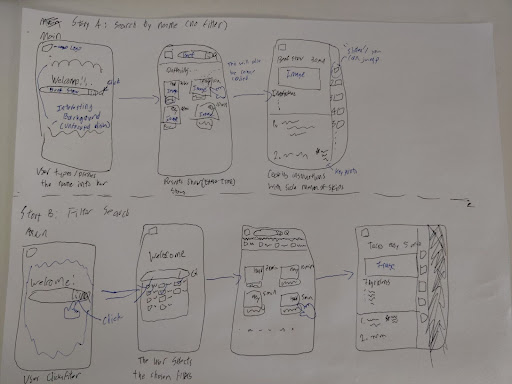
\includegraphics[width=\linewidth]{figure1.jpg}
  \caption{Takahiro's Sketch.}
  \label{fig:figure1}
\end{figure}

\begin{figure}
\centering
  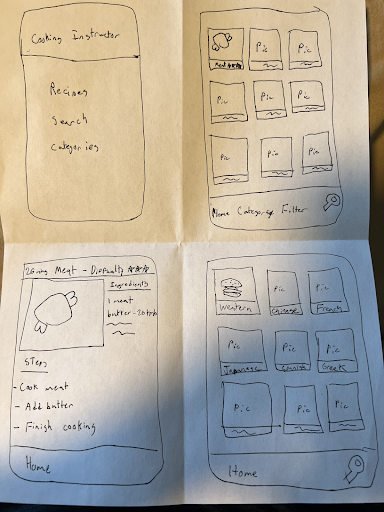
\includegraphics[width=\linewidth]{figure2.png}
  \caption{Ty's Sketch.}
  \label{fig:figure2}
\end{figure}


\begin{figure}
  \centering
  \begin{subfigure}[b]{0.4\linewidth}
    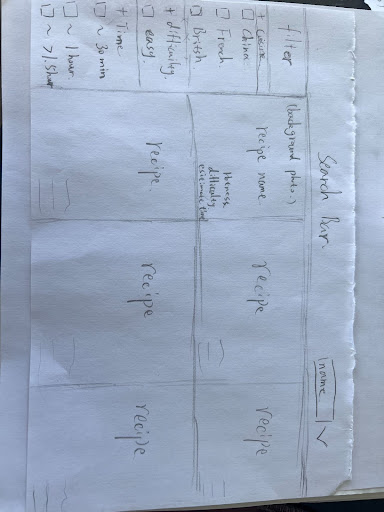
\includegraphics[width=\linewidth]{figure3v1.jpg}
    \caption{Seach Page}
  \end{subfigure}
  \begin{subfigure}[b]{0.4\linewidth}
    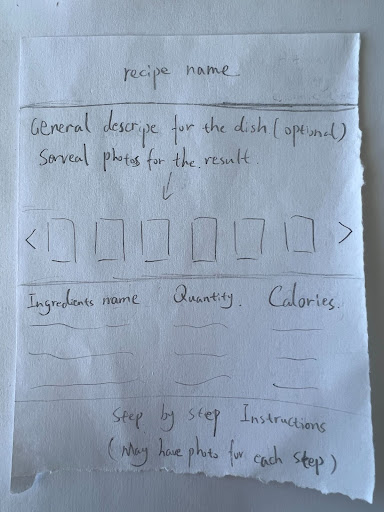
\includegraphics[width=\linewidth]{figure3v2.jpg}
    \caption{Recipe Page}
  \end{subfigure}
    \begin{subfigure}[b]{0.4\linewidth}
    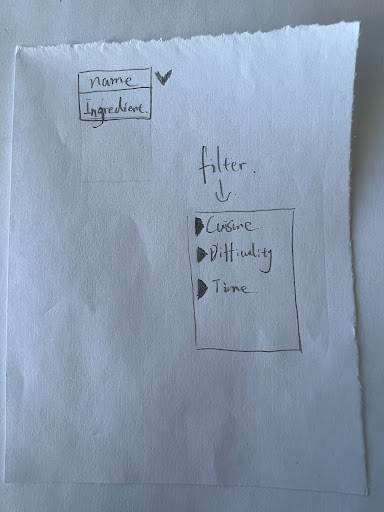
\includegraphics[width=\linewidth]{figure3v3.jpg}
    \caption{Ingredient filter}
  \end{subfigure}
  \caption{Neil's Sketch}
  \label{fig:figure3}
\end{figure}

\begin{figure}
\centering
  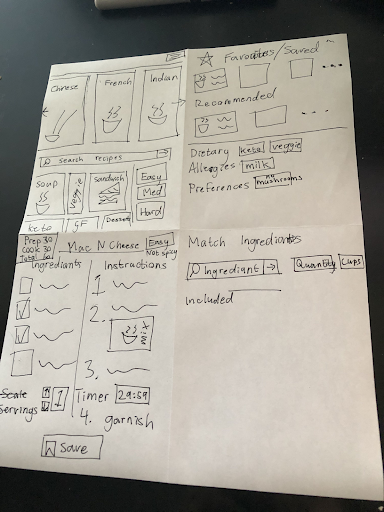
\includegraphics[width=\linewidth]{figure4.png}
  \caption{Quinn's Sketch}
  \label{fig:figure4}
\end{figure}

\begin{figure}
\centering
  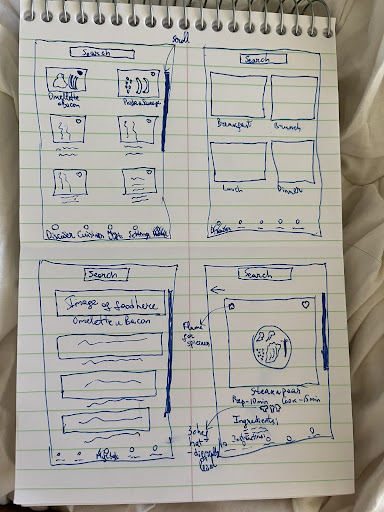
\includegraphics[width=\linewidth]{figure5.jpg}
  \caption{Elgiz's Sketch}
  \label{fig:figure5}
\end{figure}

\begin{figure}
\centering
  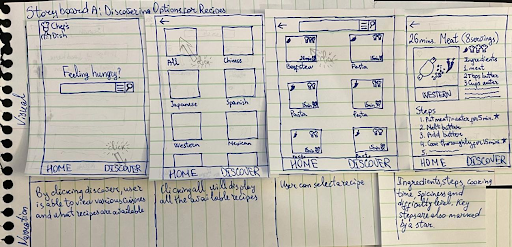
\includegraphics[width=\linewidth]{figure6v1.png}
\end{figure}

\begin{figure}
\centering
  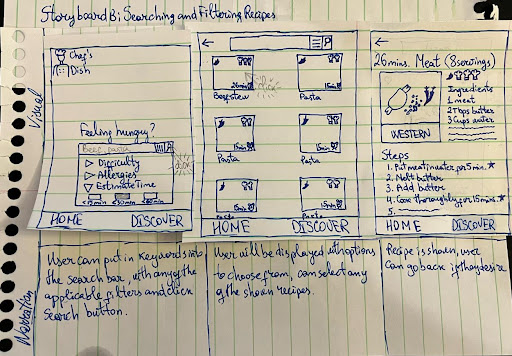
\includegraphics[width=\linewidth]{figure6v2.jpg}
  \caption{Initial Low Fidelity Prototype}
  \label{fig:figure6}
\end{figure}

\begin{figure}
\centering
  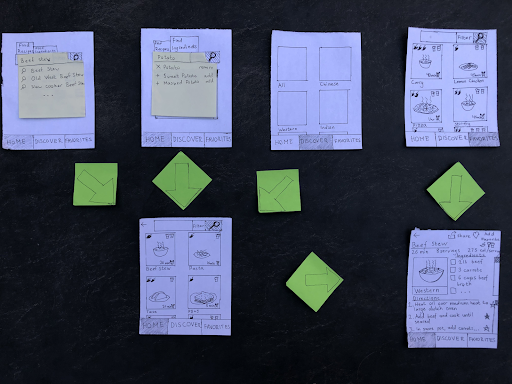
\includegraphics[width=\linewidth]{figure7.png}
  \caption{Final Low Fidelity Prototype}
  \label{fig:figure7}
\end{figure}

\begin{figure}
  \centering
  \begin{subfigure}[b]{0.4\linewidth}
    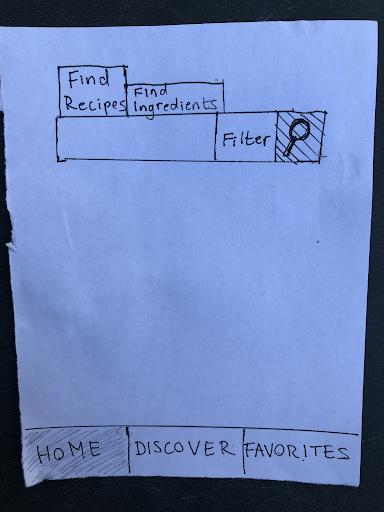
\includegraphics[width=\linewidth]{figure8v1.png}
  \end{subfigure}
  \begin{subfigure}[b]{0.4\linewidth}
    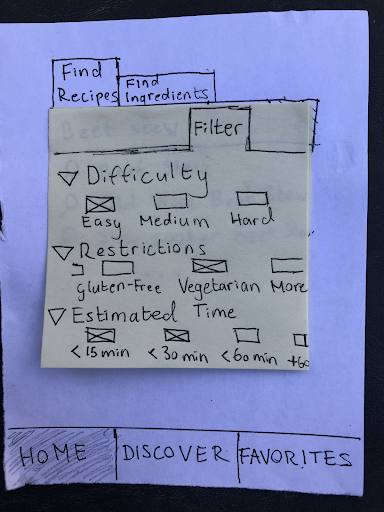
\includegraphics[width=\linewidth]{figure8v2.png}
  \end{subfigure}
    \begin{subfigure}[b]{0.4\linewidth}
    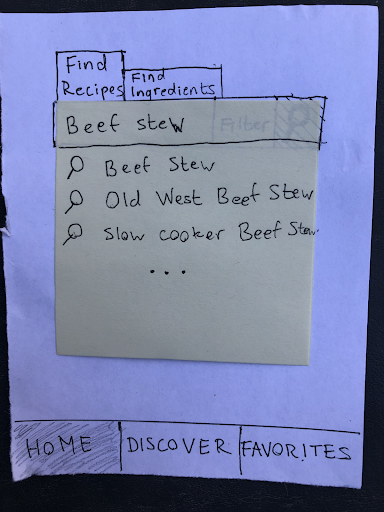
\includegraphics[width=\linewidth]{figure8v3.png}
  \end{subfigure}
  \caption{`Find Recipe` Pictive Prototype}
  \label{fig:figure8}
\end{figure}

\begin{figure}[H]
  \centering
  \begin{subfigure}[b]{0.4\linewidth}
    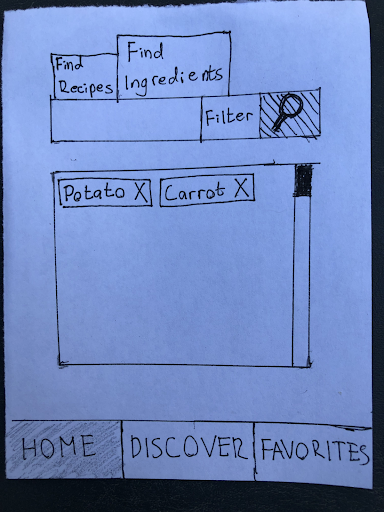
\includegraphics[width=\linewidth]{figure9v2.png}
  \end{subfigure}
  \begin{subfigure}[b]{0.4\linewidth}
    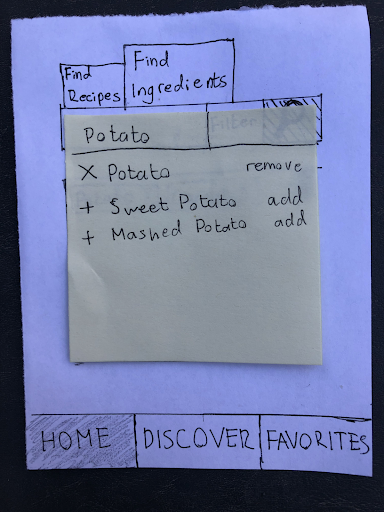
\includegraphics[width=\linewidth]{figure9v1.png}
  \end{subfigure}
  \caption{`Find Ingredients' Pictive Prototype}
  \label{fig:figure8}
\end{figure}
\newpage
\newpage
\section{Appendix B: Grading Sheet}
\subsection{Structure and Format}
\begin{longtable}{>{\hspace{0pt}}m{0.148\linewidth}>{\hspace{0pt}}m{0.181\linewidth}>{\hspace{0pt}}m{0.262\linewidth}>{\hspace{0pt}}m{0.248\linewidth}>{\hspace{0pt}}m{0.098\linewidth}}
 & \textbf{Included} & \textbf{Not Included} &  &  \endfirsthead
 &  &  &  &  \\
Portfolio in PDF & 1 & 0 &  &  \\
Section separators & 1 & 0 &  &  \\
Name on outside cover & 1 & 0 &  &  \\
Name and contact information on the first page & 1 & 0 &  &  \\
This grading sheet included in portfolio & 4 & 0 &  &  \\
 & \textbf{Complete} & \textbf{Missing portions~} & \textbf{Not included} &  \\
Table of contents & 2 & 1 & 0 &  \\
 & \textbf{Great: no problems~} & \textbf{Good: a few minor problems~} & \textbf{Poor: Problems throughout (your mark in other sections may also be affected as well)} &  \\
Appearance (organization, layout and whitespace) & 6 & 4 & 0 &  \\
 & \textbf{No typos, grammatical or spelling errors, clear writing style} & \textbf{Minor typos or grammatical errors or spelling mistakes or some writing may be a bit vague} & \textbf{Problems in two areas (spelling, grammar, style)} & \textbf{Problems in all three areas} \\
Language and writing style & 7 & 5 & 3 & 0
\end{longtable}
\subsection{Setting the stage}

\begin{longtable}{>{\hspace{0pt}}m{0.25\linewidth}>{\hspace{0pt}}m{0.285\linewidth}>{\hspace{0pt}}m{0.238\linewidth}>{\hspace{0pt}}m{0.135\linewidth}>{\hspace{0pt}}m{0.025\linewidth}}
 & \textbf{Clear and complete (yes)} & \textbf{Clear and complete (no)} &  &  \endfirsthead
Background & 1 & 0 &  &  \\
Expected uses of the system~ & 1 & 0 &  &  \\
System constraints & 1 & 0 &  &  \\
 & \textbf{Lists user groups along with relevant skills and experience} & \textbf{Lists user groups with no additional information} & \textbf{Information not included} &  \\
Expected users & 2 & 1 & 0 &  \\
 & \textbf{Clear \& complete} & \textbf{Some information missing or unclear} & \textbf{Information not included} &  \\
Work context & 2 & 1 & 0 &  \\
 & \textbf{Spoke directly with actual users} & \textbf{Spoke with a representative of the user} & \textbf{Made it all up} &  \\
Approach for getting background information for tasks & 2 & 1 & 0 & 
\end{longtable}

\subsection{Requirements}

\begin{longtable}{>{\hspace{0pt}}m{0.131\linewidth}>{\hspace{0pt}}m{0.279\linewidth}>{\hspace{0pt}}m{0.267\linewidth}>{\hspace{0pt}}m{0.177\linewidth}>{\hspace{0pt}}m{0.081\linewidth}}
 & \textbf{Requirements are grouped into categories with clear and detailed explanations based on the users and their tasks~} & \textbf{Requirements are grouped into categories, no indication of how functions were put into particular categories} & \textbf{Requirements are shown in a single list, no attempt at prioritization~} & \textbf{No requirements listed} \endfirsthead
Description of system functions to be implemented & 5 & 2 & 1 & 0
\end{longtable}

\subsection{Tasks}

\begin{longtable}{>{\hspace{0pt}}m{0.208\linewidth}>{\hspace{0pt}}m{0.137\linewidth}>{\hspace{0pt}}m{0.24\linewidth}>{\hspace{0pt}}m{0.177\linewidth}>{\hspace{0pt}}m{0.175\linewidth}}
 & \textbf{Appropriate No. (\textasciitilde{}5-7)} & \textbf{Fewer than what's needed for the usage of the system} & \textbf{No tasks were included in the portfolio} &  \endfirsthead
Number of tasks & 2 & 1 & 0 &  \\
 & \textbf{Covers all relevant activities} & \textbf{Missing a few important tasks~} & \textbf{Missing many important tasks} & \textbf{No tasks were included in the portfolio} \\
Coverage of the tasks & 8 & 6 & 2 & 0 \\
 & \textbf{No violations} & \textbf{A few minor violations Many violations throughout} & \textbf{Many violations throughout} & \textbf{No tasks were included in the portfolio} \\
Do the tasks follow the properties of a good task? & 8 & 6 & 2 & 0
\end{longtable}

\subsection{Prototypes}

\begin{longtable}{>{\hspace{0pt}}m{0.171\linewidth}>{\hspace{0pt}}m{0.315\linewidth}>{\hspace{0pt}}m{0.256\linewidth}>{\hspace{0pt}}m{0.194\linewidth}}
 & \textbf{Two or more} & \textbf{One} &  \endfirsthead
Number of versions/iterations~ & 2 & 1 &  \\
 & \textbf{Marked improvement from version to version~} & \textbf{Few and/or superficial changes from version to version~} & \textbf{No evolution between prototype versions} \\
Evolution of prototypes & 6 & 2 & 0 \\
 & \textbf{Provides clear idea of how prototype changed from version to version~} & \textbf{Describes changes but some parts are unclear~} & \textbf{None} \\
Description of how prototypes evolved & 4 & 2 & 0
\end{longtable}

\subsection{Walkthroughs}

\begin{longtable}{>{\hspace{0pt}}m{0.108\linewidth}>{\hspace{0pt}}m{0.235\linewidth}>{\hspace{0pt}}m{0.306\linewidth}>{\hspace{0pt}}m{0.208\linewidth}>{\hspace{0pt}}m{0.079\linewidth}}
 & \textbf{Walkthroughs for all relevant tasks~} & \textbf{One} & \textbf{Zero} &  \endfirsthead
Number of walkthroughs performed & 4 & 1 & 0 &  \\
 & \textbf{Walkthroughs conducted, all or most usability problems were caught} & \textbf{Walkthroughs conducted, some minor problems were missed} & \textbf{Walkthroughs conducted, many minor or several serious problems were missed} & \textbf{Walkthrough not performed} \\
Results of conducting the walkthrough algorithm & 10 & 8 & 4 & 0 \\
 & \textbf{Walkthrough results summarized for each scenario/task~}\par{}\textbf{An analysis conducted that summarized for all tasks what are the high level and major problems} & \textbf{Walkthrough results summarized for each scenario/task but not for all tasks} & \textbf{Walkthroughs conducted and results shown in table but no additional analysis, summarizing problems} &  \\
Analysis of walkthrough results & 6 & 3 & 0 &  \\
 & \textbf{Walkthroughs easy to follow (e.g., included diagrams at all relevant points of walkthrough, diagrams are annotated)} & \textbf{Some points of the walkthrough difficult to follow (e.g., walkthrough description didn't match interface, additional diagrams would have made things clearer)} & \textbf{Walkthroughs not conducted~} &  \\
Ease of following/tracing the walkthroughs & 6 & 3 & 0 & 
\end{longtable}

\subsection{Tutorial Presentations}

\begin{longtable}{>{\hspace{0pt}}m{0.137\linewidth}>{\hspace{0pt}}m{0.185\linewidth}>{\hspace{0pt}}m{0.248\linewidth}>{\hspace{0pt}}m{0.225\linewidth}>{\hspace{0pt}}m{0.142\linewidth}}
 & \textbf{Provides clear background information, good tasks presented, requirements properly categorized~} & \textbf{Minor problems: some background information unclear, minor violations in the descriptions of the tasks, requirements could better justified~} & \textbf{Poor: task violate many properties of good tasks, or background missing or largely incomplete, requirements are not justified} & \textbf{No presentation} \endfirsthead
First presentation: Phase one and two~ & 4 & 3 & 1 & 0 \\
 & \textbf{Walkthrough: caught most problems, clear indication of what future improvements should be}\par{}\textbf{Prototype: Gives a good feel for how the interaction unfolds, covers main system functions~} & \textbf{Walkthrough: Missed a few minor problems in the walkthrough~}\par{}\textbf{Prototype: Some parts of the interaction unclear, a few minor system functions (relevant to task) or a major function is missing~} & \textbf{Walkthrough: Missed many minor problems in the walkthrough or a few major usability problems~}\par{}\textbf{Prototype: several main system functions missing~} & \textbf{Walkthrough: Many serious problems were missed in the walkthrough~}\par{}\textbf{Prototype: main system functions were missing} \\
Second presentation: Phase three  four & 4 & 3 & 1 & 0 \\
 &  &  &  &  \\
All team members completed all weekly MVP surveys to portfolio due date & Complete & Incomplete &  & 
\end{longtable}




\end{document}